%==============================
\subsection{Simulations and Experiment}\label{subsec:simulation}


The numerical study simulates a team of multiple UGVs and UAVs
that are responsible for maintaining a remote photovoltaic (PV) power station.
We first describe the scenario and three types of tasks,
followed by the results obtained via the proposed method.
Then, we introduce various changes in the environment and agent failures,
in order to validate the proposed online adaptation algorithm.
Third, we perform scalability analysis of our method by increasing
the system size and the task complexity.
Lastly, we compare our methods against several strong baselines, in terms of
optimality, computation time and adaptation efficiency.


%==============================
\begin{figure}
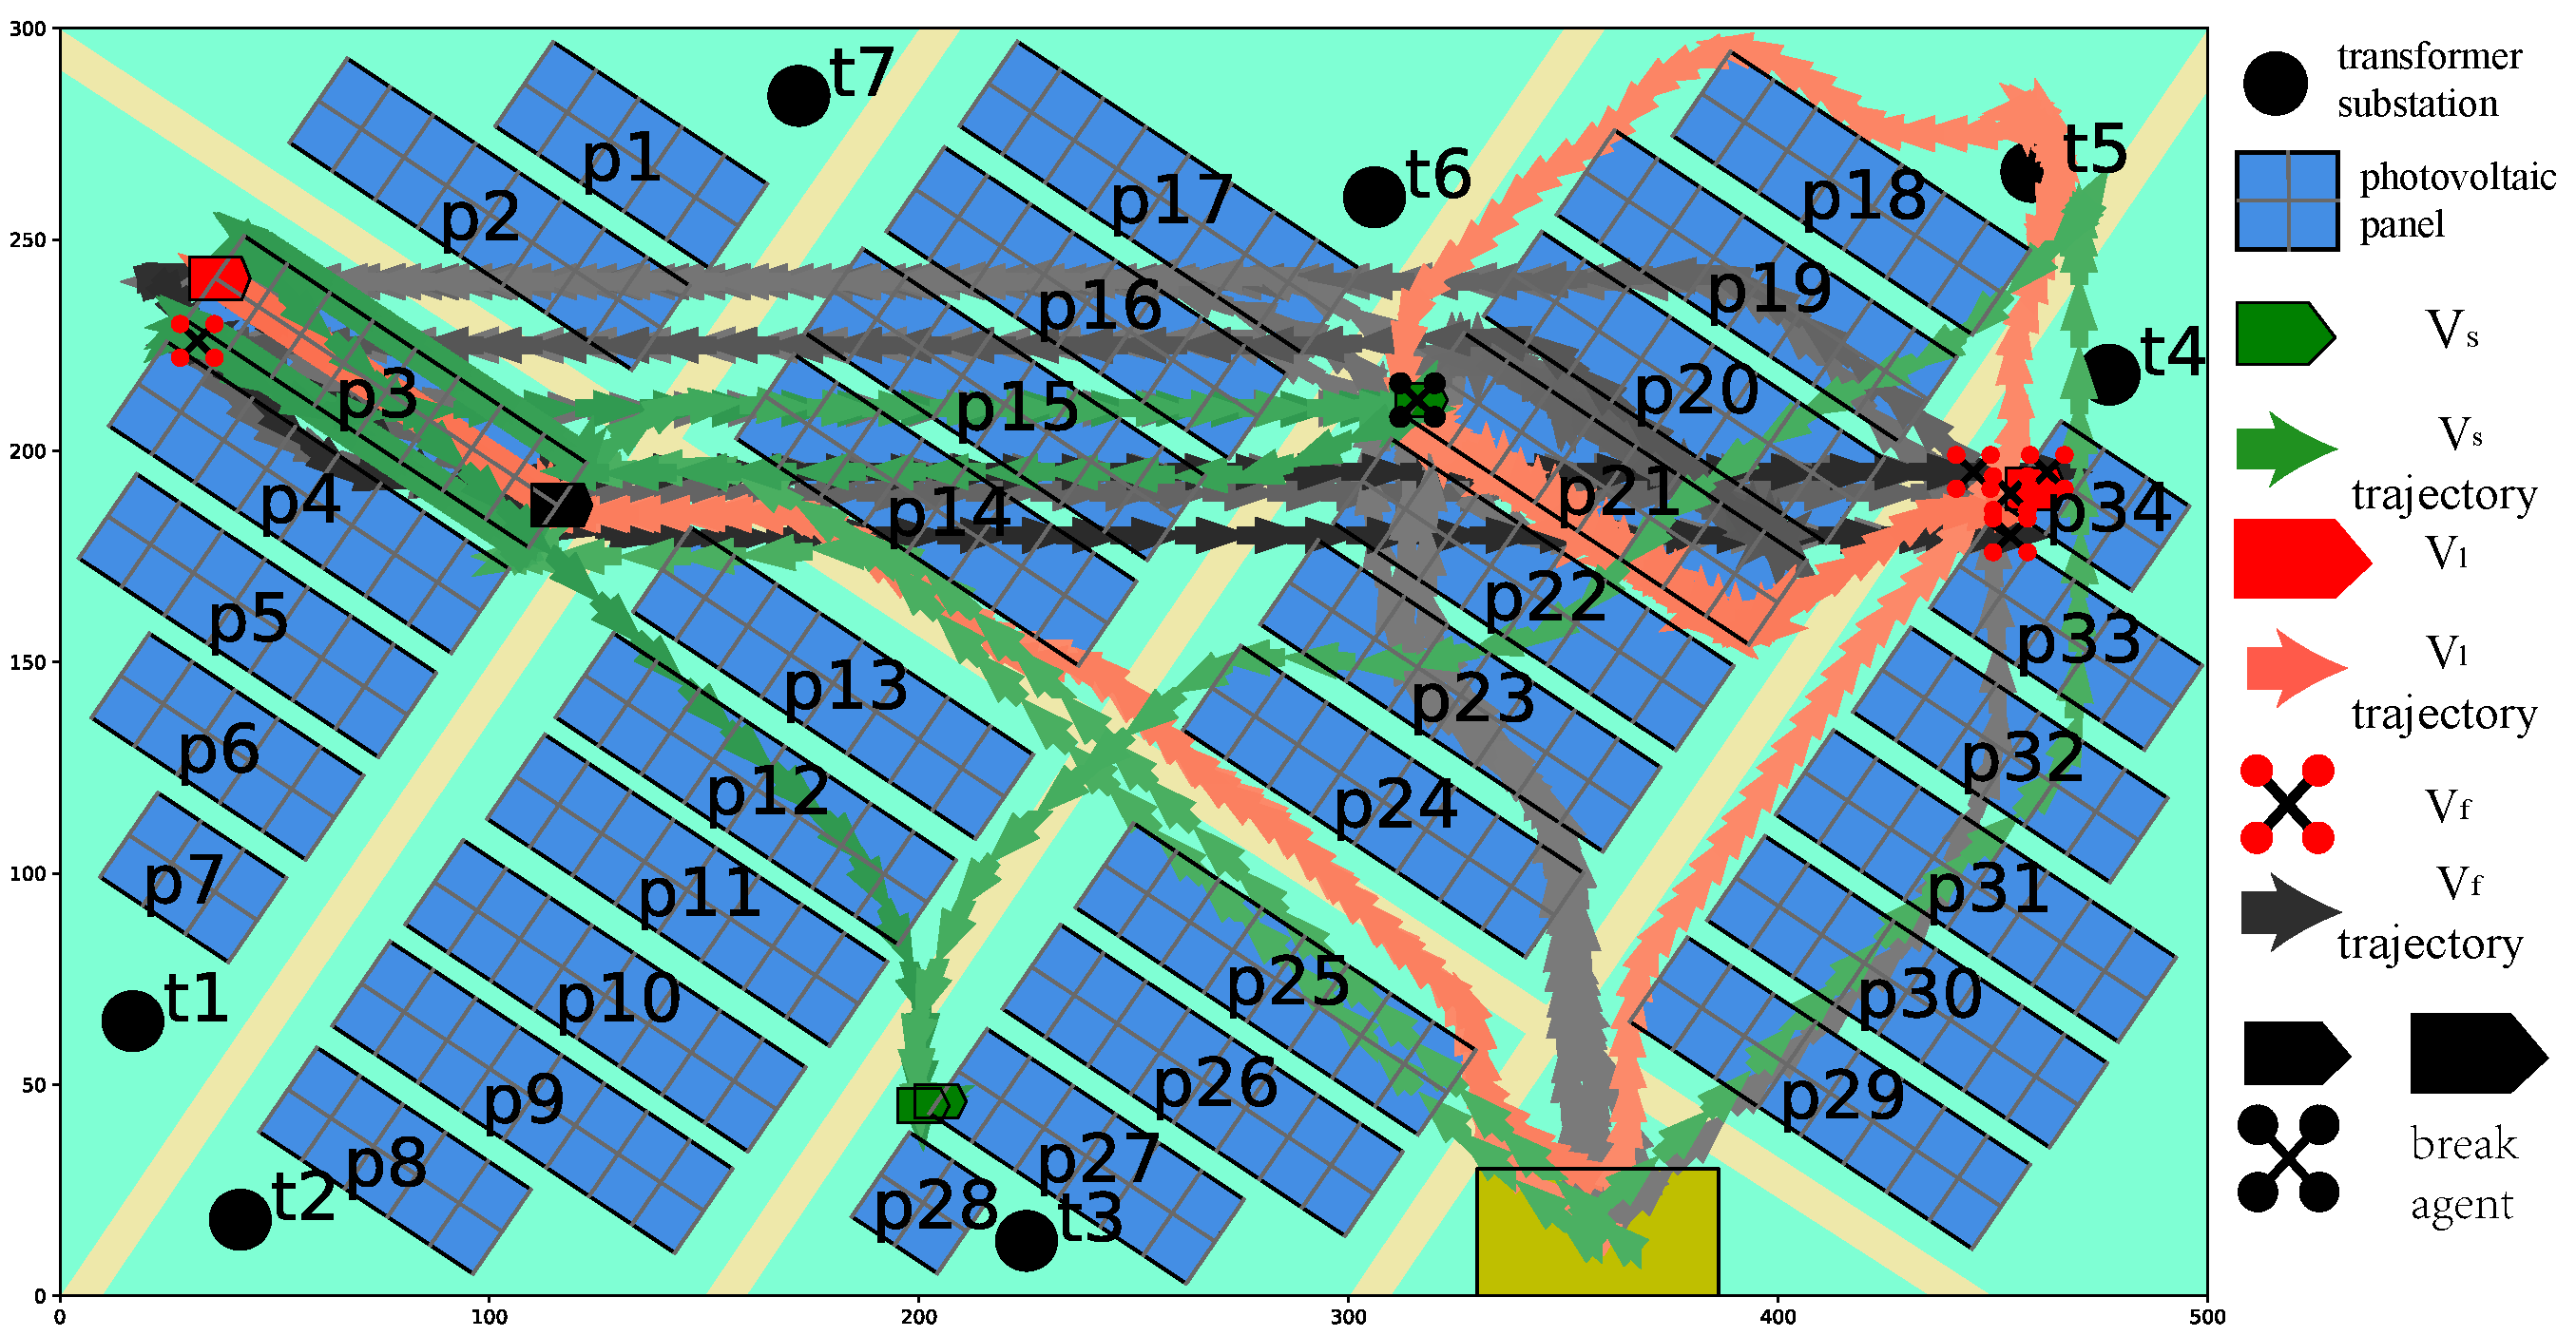
\includegraphics[scale=0.18]{figures/background3.pdf}
\caption{PV power station in the numerical simulation study,
  which consists of PV panels~$\texttt{p}_i$, roads,
  inverters/transformers~$\texttt{t}_i$ and base stations~$b$.
  The arrow trajectories are the paths of the agents 
  executing the LTL formula~$\varphi_{1}$. The arrow direction
  is the motion direction and the arrow density correspond to the velocity of different agents.}
\label{fig:workspace}
\end{figure}
%==============================


%===========================
  \begin{figure*}
    \centering
        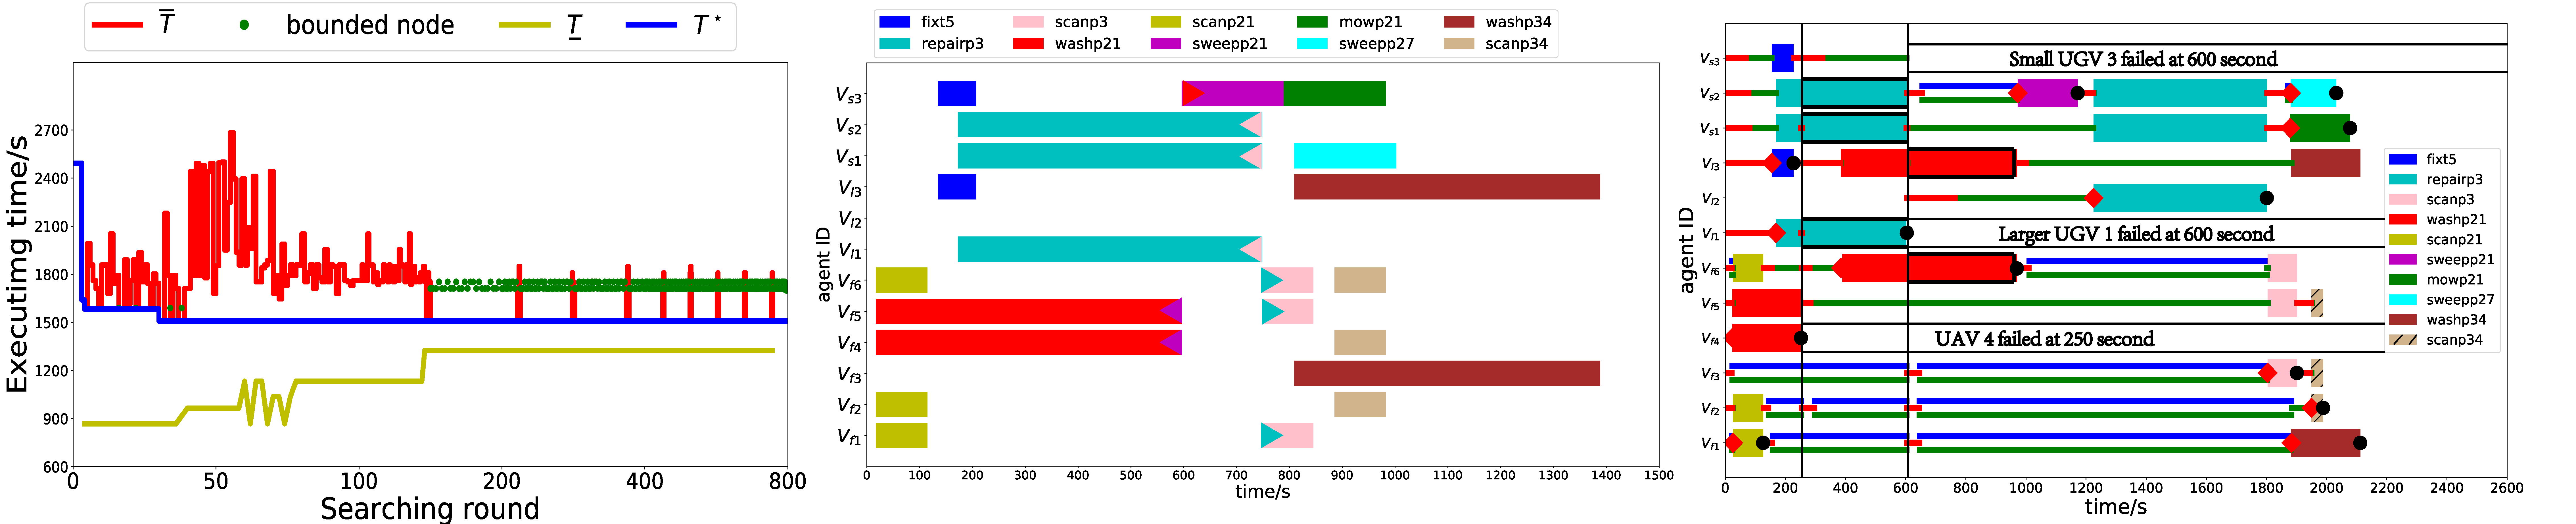
\includegraphics[width=1\textwidth]{figures/simulation/taskfinal/mixed_poset.pdf}
    \caption{\textbf{Left}: Illustration of the upper and lower
bounds~$\overline{T}_\nu,\,\underline{T}_\nu$, and the optimal value~$T^\star$,
along with the BnB search process.
\textbf{Middle}: Gantt graph of offline planning.
\textbf{Right}: Gantt graph of the plan execution under agent failures and fluctuated subtask duration during the execution.
Additional lines and labels are added to highlight the online synchronization process. Red segments denote that the agents
are during transition among regions, green seqments denote "communicate
with collaborate leader", and blue segments denote
``leader communicate with other leader for \texttt{start} and \texttt{stop} messages”.
The ``\texttt{start}" message is marked by the red diamond and the ``\texttt{stop}" message
by the black dot, both of which are published by the respective leader.
Three agent failures are highlighted in black.
    }
\label{fig:task2-bnb}
\end{figure*}
  %===========================

%==============================
\subsubsection{Workspace Description}\label{subsubsec:ws}

Consider a group of UAVs and UGVs working in a PV power station for
long-term daily maintenance.
As shown in Fig.~\ref{fig:workspace},
the station consists of mainly three parts: PV panels $\texttt{p}_1,\cdots,\texttt{p}_{34}$, roads,
inverter/transformer substations $\texttt{t}_1,\cdots,\texttt{t}_7$ and the robot base station $\texttt{b}$.
Furthermore, there are one type of UAVs and two types of UGVs.
The UAVs $V_f$ are quadcopters which can move freely between all interested places.
The larger type of UGVs, denoted by $V_l$, has the limitation of not going to PV panels or transformers;
the smaller ones $V_s$ can travel more freely, e.g., under the PV panels but not under the transformers.
As a result, different types of robots have different motion
models~$\mathcal{G}_n$ as described in Sec.~\ref{subsec:multi-agent}
and distinctive action models.
The traveling time among the regions of interest is estimated by the route
distance and their respective speed.
Detailed descriptions of the workspace and robot model are omitted here due to limited space. 
Interested readers please refer to \citep{liu2022arxiv}.
Note that some actions can be performed alone while some require direct
collaboration of several agents,
e.g., one $V_s$ can $sweep$ debris under the PV panel while one $V_l$
and two $V_s$ are required to $repair$ a broken PV panel.







%==============================
\subsubsection{Task Description}\label{subsubsec:task}



%% \begin{table}[t]\footnotesize
%% \caption{definition of agent with function}
%% \label{table:agent}
%% \begin{tabular}{|c|c|c|c|}\hline
%% 	\textbf{Agent type} &\textbf{label} & \textbf{Capable action} & \textbf{Speed}$(m/ s )$\\ \hline
%% 	 Quadcopter& $V_f$  & $temp, scan, wash $ & 10 \\ \hline
%% 	 Larger UGV& $V_l$  & $wash,repair_l,fix$ & 4 \\ \hline
%% 	 Smaller UGV& $V_s$  &  $sweep, mow, repair_s, fix$ & 4 \\ \hline
%% \end{tabular}
%% \end{table}


%% %==============================
%% \begin{table}[t]\footnotesize
%%  \centering
%% \caption{Description of related regions and agent actions.}
%% \label{fig:symbols}
%% \begin{tabular}{|c|m{0.5\columnwidth}|c|}\hline
%% \textbf{Proposition} & \textbf{Description}\centering & \textbf{Duration} [s]\\ \hline
%% $\texttt{p}_1,\cdots,\texttt{p}_{34}$ & $34$ PV panels. & $\backslash$ \\ \hline
%% $\texttt{b}$ & Base stations for all agents to park and charge. & $\backslash$ \\ \hline
%% $\texttt{t}_1,\cdots,\texttt{t}_7$ & $7$ transformers. & $\backslash$ \\ \hline
%% $\texttt{temp}_{\texttt{p}_i,\texttt{t}_i}$ &
%% Measure temperature of panel~$\texttt{p}_i$ and transformer $\texttt{t}_i$.
%% Requires 1 $temp$ action. & 10 \\ \hline
%% $\texttt{sweep}_{\texttt{p}_i}$& Sweep debris around any panel~$\texttt{p}_i$.
%% Requires 1 $sweep$ action. & 190\\ \hline
%% $\texttt{mow}_{\texttt{p}_i,\texttt{t}_i}$ &
%% Mow the grass under panel~$\texttt{p}_i$ or transformer~$\texttt{t}_i$.
%% Requires 1 $mow$ action. & 190\\ \hline
%% $\texttt{fix}_{\texttt{t}_i}$ &
%% Fix malfunctional transformer~$\texttt{t}_i$.
%% Requires 2 $fix$ action collaborations & 72\\ \hline
%% $\texttt{repair}_{\texttt{p}_i}$ &
%% Repair broken panel~$\texttt{p}_i$.
%% Requires 2 $repair_s$,1 $repair_l$ action collaborations . & 576\\ \hline
%% $\texttt{wash}_{\texttt{p}_i}$ &
%% Wash the dirt off panel~$\texttt{p}_i$.
%% Requires 2 $wash$ actions collaborations. & 565\\ \hline
%% $\texttt{scan}_{\texttt{p}_i,\texttt{t}_i}$ &
%% Build 3D models of panel~$\texttt{p}_i$ or transformer~$\texttt{t}_i$
%% for inspection. Requires 3 $scan$ action. & 95\\ \hline
%% \end{tabular}
%% \end{table}
%% %==============================

For the nominal scenario, we consider a system of moderate size,
including $12$ agents: 6 $V_f$, 3 $V_l$ and 3 $V_s$.
Scalability analyses to larger systems are performed later in Sec.~\ref{subsubsec:scalable}.
Moreover, we consider a complex task and test it with agent failure.
This task can be specified as the following LTL formulas,
requires a series of limited actions to
maintain the photovoltaic power station:
\begin{equation}\footnotesize
\label{eq:task1}
  \begin{aligned}
\varphi_1 = & \Diamond(\texttt{repair}_{\texttt{p}_{3}} \wedge \lnot \texttt{scan}_{\texttt{p}_3} \wedge\Diamond \texttt{scan}_{\texttt{p}_3})
\wedge \Diamond (\texttt{wash}_{\texttt{p}_{21}} \wedge \\
&\Diamond \texttt{mow}_{\texttt{p}_{21}} \wedge \Diamond \texttt{scan}_{\texttt{p}_{21}}) \wedge \Diamond ( \texttt{sweep}_{\texttt{p}_{21}} \wedge \lnot \texttt{wash}_{\texttt{p}_{21}} \wedge\\
& \Diamond \texttt{mow}_{\texttt{p}_{21}}) \wedge \Diamond(\texttt{fix}_{\texttt{t}_5} \wedge \lnot \texttt{p}_{\texttt{18}}) \wedge \lnot \texttt{p}_{24} \,U \, \texttt{sweep}_{\texttt{p}_{27}} \\
&\wedge \Diamond (\texttt{wash}_{\texttt{p}_{34}} \wedge \bigcirc \texttt{scan}_{\texttt{p}_{34}}),
\end{aligned}
\end{equation}
where the locations of these subtasks are chosen across the workspace.
Thus, a strategy to minimize the completion time is crucial.

%========================================
\subsubsection{Results}\label{subsubsec:results}
In this section, we present the results of the proposed method, including the computation of R-posets,
task assignment via the BnB search algorithm, and the task execution.

%===========================
\begin{figure}[t!]
		\centering%
		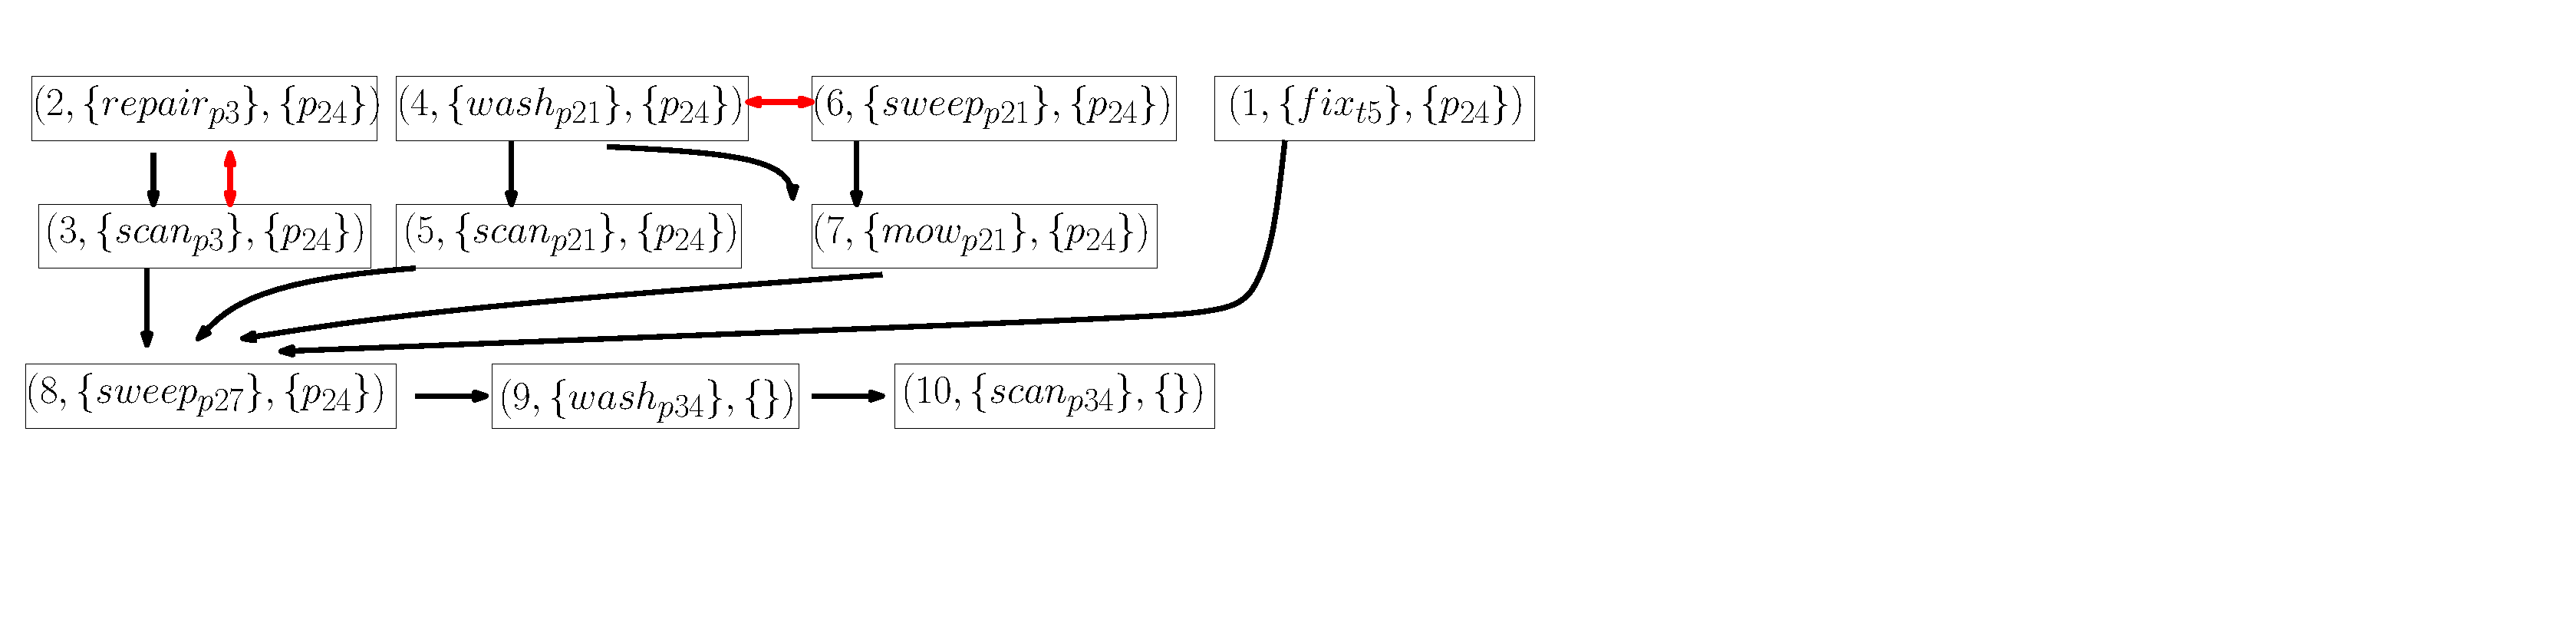
\includegraphics[height = 0.12 \textwidth]{figures/simulation/taskfinal/ipe_poset_graph.pdf}
	\caption{R-Poset graph of task $\varphi_1$, in which the negative labels of $\sigma_\ell$ are omitted here for simplicity.
          The relations~$\preceq_\varphi,\, \neq_{\varphi}$ are marked
          by black and red arrows.}
       \label{fig:task12-posets}
\end{figure}
%===========================

\textbf{Partial analysis}:
The NBA~$\mathcal{B}_{\varphi_1}$ associated with task $\varphi_1$ in~\eqref{eq:task1}
contains~$707$ states and~$16044$ edges. And the pruning step reduces $84.9\%$ edges within
$30.43$ second. Then, the Alg.~\ref{alg:compute-poset} explores
 $4$ accepting runs in $0.14s$ to find the first R-poset and gets the best R-poset in $22.40s$.
 Finally, as showed in Fig. \ref{fig:task12-posets}, we choose the best R-poset $P^{p}_{\varphi}$ with $10$ subtasks, whose language
 $L(P^{p}_{\varphi})$ has $525$ {words}. In $P^{p}_{\varphi}$, there are
 multiple subtasks that can be executed in parallel such as $\omega_2 $ with $ \omega_4$, $\omega_1 $ with $ \omega_7$.
 However, these subtasks are still ordered as no subtask set can be executed independent with the left
 subtasks. This means that we cannot
 divide the word into a series of independent parts using the method in \citep{schillinger2018simultaneous}.
 It is worth noting that this R-poset has only one subtask $\omega_7$ with $\texttt{mow}_{\texttt{p}_{21}}$,
 which is required twice in $\varphi_1$. It follows additional partial orders as
 $\omega_4\preceq_\varphi \omega_8,\omega_6\preceq_\varphi \omega_8$. This means that our method can find
 a more efficient R-poset with relations not explicitly written in the formula.
 There are two $\neq_\varphi$ relations $(\omega_2,\omega_3),(\omega_4,\omega_6)$, due to the constrains
 $\texttt{repair}_{\texttt{p}_3}\wedge\lnot\texttt{scan}_{\texttt{p}_3} $ and
  $\texttt{sweep}_{\texttt{p}_{21}} \wedge \lnot \texttt{wash}_{\texttt{p}_{21}}$ in formula $\varphi_1$.
  Until execute $\omega_8$, all subtasks have the labels of self loop  $\lnot p_{24}$ due to
   $\lnot \texttt{p}_{24} U \texttt{sweep}_{\texttt{p}_{27}}$.



%% %===========================
%% \begin{figure}[t!]
%% \centering%
%% 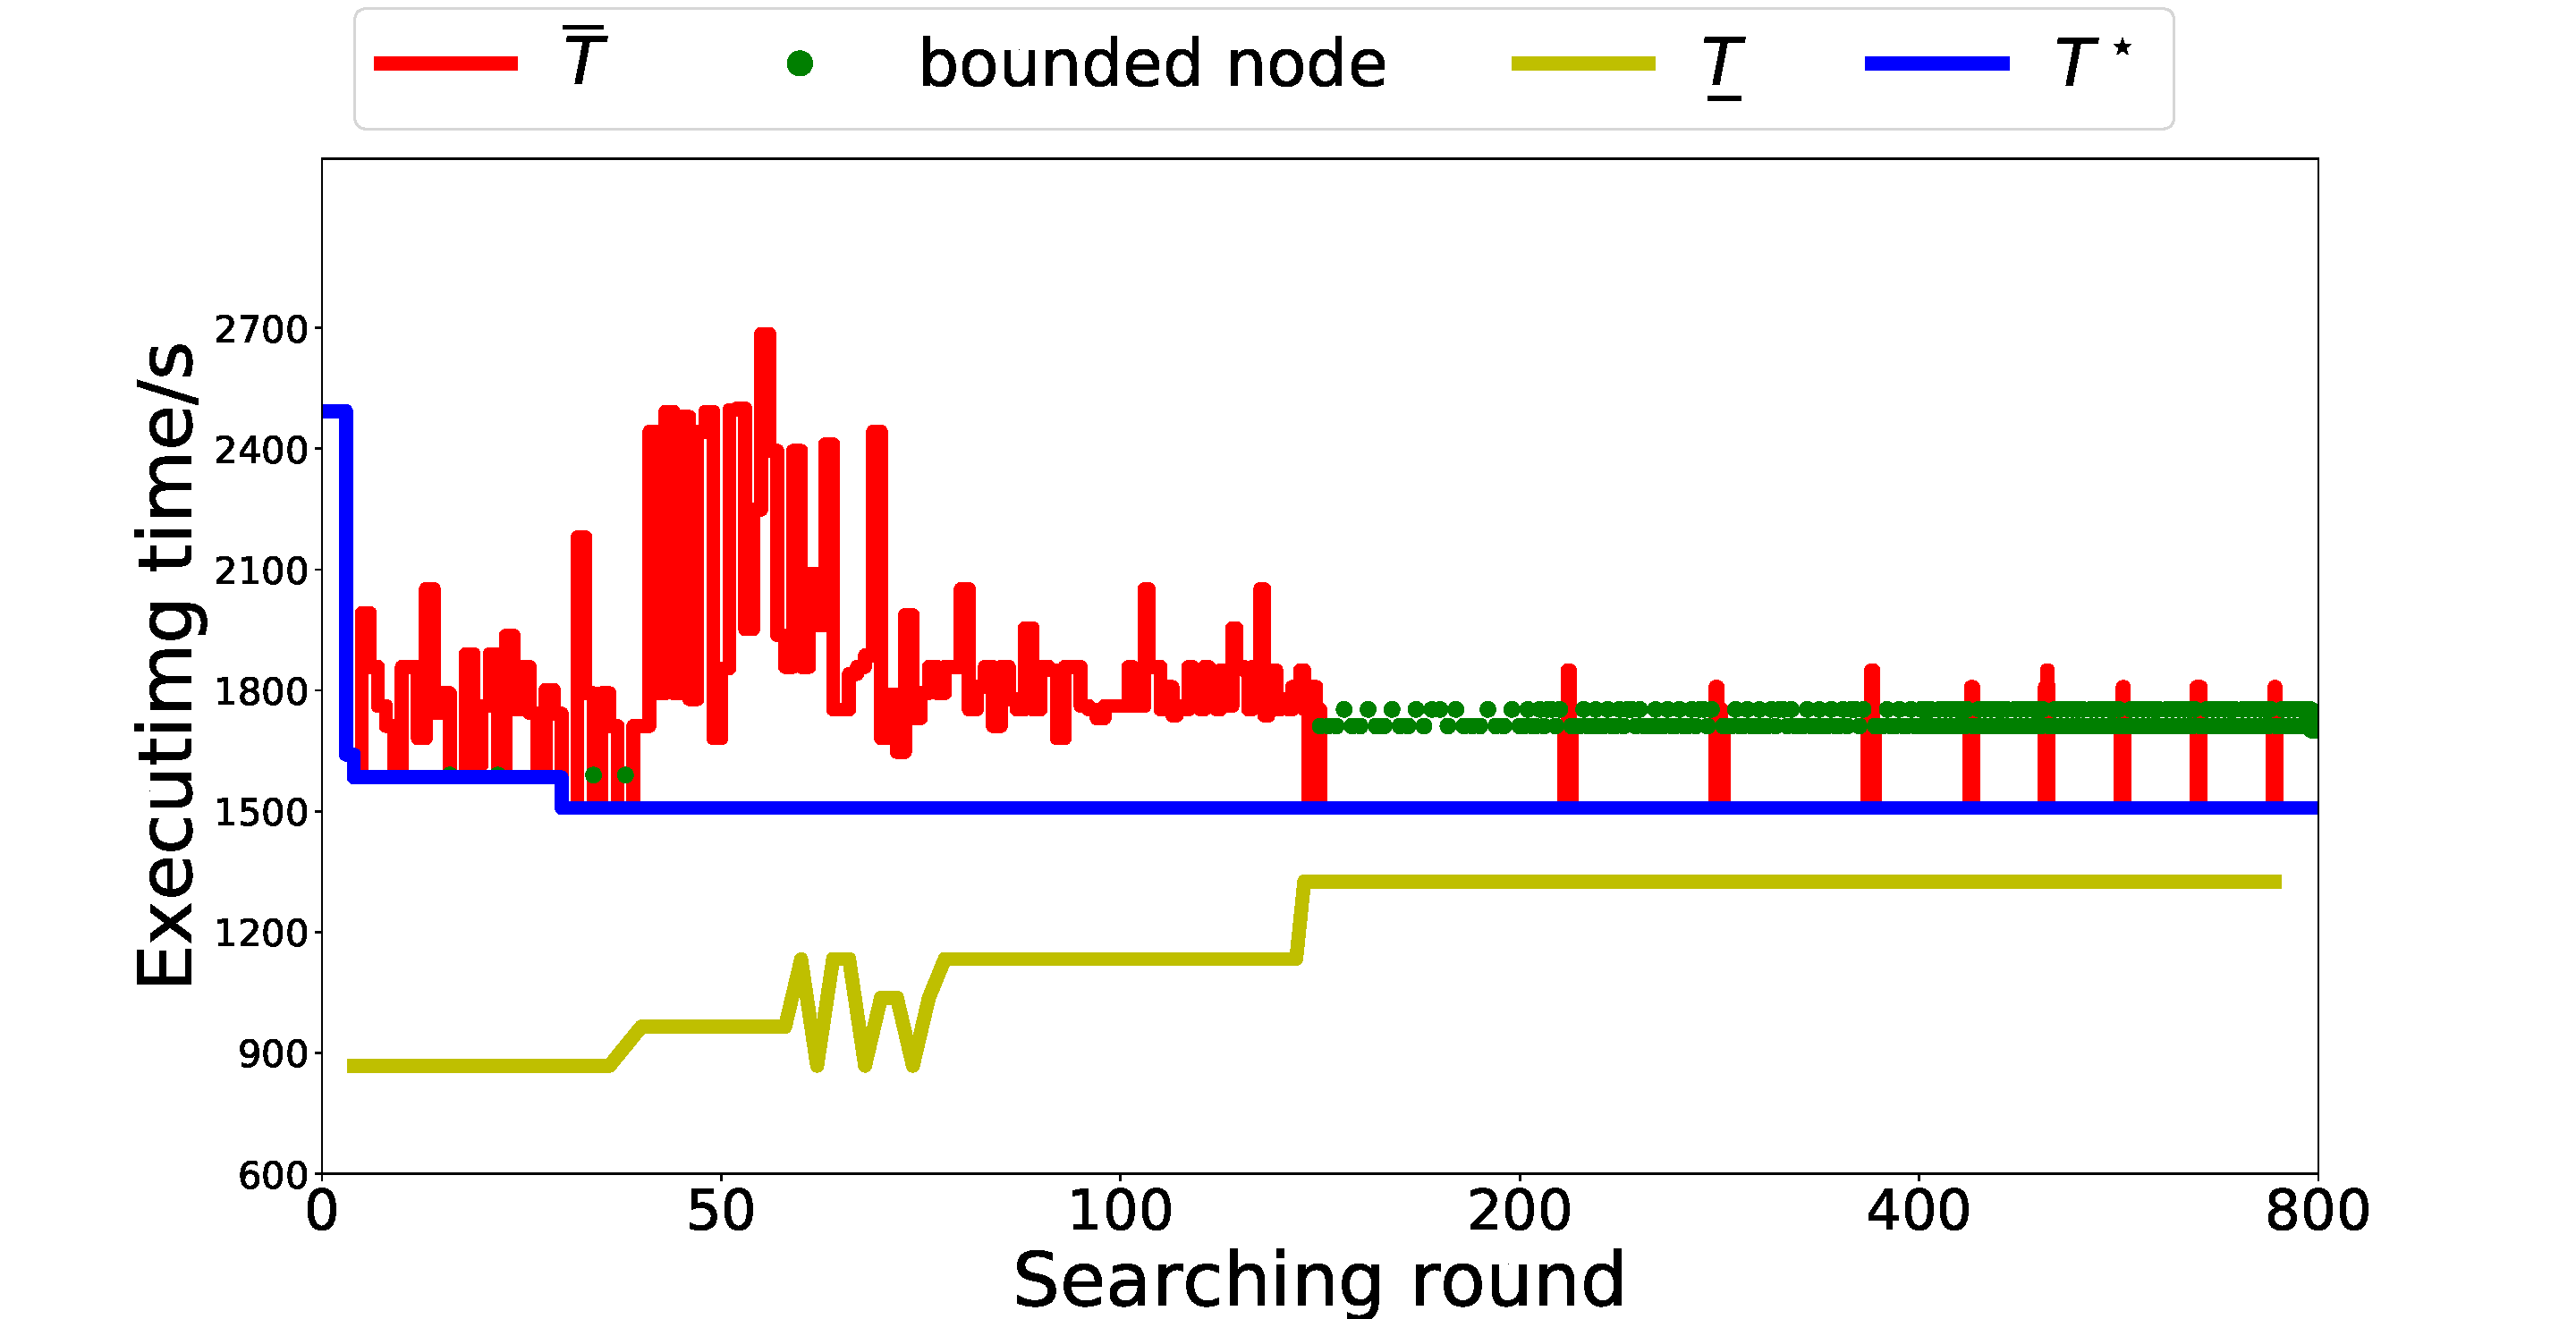
\includegraphics[width = 0.50\textwidth]{figures/simulation/taskfinal/bnb.pdf}
%% \caption{Illustration of the upper and lower
%% bounds~$\overline{T}_\nu,\,\underline{T}_\nu$, and the optimal value~$T^\star$,
%% along with the BnB search process.}
%% \label{fig:task2-bnb}
%% \end{figure}
%% %===========================
\textbf{Task assignment}:
Then, during the task assignment step,
the first valid solution is found in~$0.131s$.
Afterwards, at~$t=1.75s$, a node is reached and its estimated lower
bound is larger than the current upper bound, and thus cut off from the search tree.
Overall, around~$84.2\%$ of visited nodes are cut off,
which clearly shows the benefits of the ``bounding'' mechanism.
Then, the estimated upper bound rapidly converges
to the optimal $T^\star=1388.5s$ in~$3.34s$ by exploring~$30$ nodes.
This is due to the branching efficiency during the BnB search,
using the estimated lower bounds as heuristics.
Lastly, the whole search tree is exhausted after more than~$10$ hours,
due to the complexity of the problem.


As shown in Fig.~\ref{fig:task2-bnb},
in the optimal task assignment, for the same type of task $\texttt{wash}$,
different types of agent $V_{f3},V_{l3}$ are employed for $\texttt{wash}_{\texttt{p}_{34}}$ and
 $V_{f4},V_{f5}$ for $\texttt{wash}_{\texttt{p}_{21}}$. All the constraints
 of $\preceq_\varphi,\neq_\varphi$ are satisfied, e.g., $\texttt{mow}_{\texttt{p}_{21}}$
should be executed after $\texttt{wash}_{\texttt{p}_{21}}$,
$\texttt{sweep}_{\texttt{p}_{21}}$ and $\texttt{wash}_{\texttt{p}_{21}}$
should not be executed at the same time. These relations are denoted by triangles of the corresponding color.
Moreover, most subtasks without these relations are executed in parallel, such as $\omega_1,\omega_2$.
These parallelisms dramatically reduce the makespan.
%In Fig.~\ref{fig:workspace}, the self-loop labels of each subtasks are all avoided,
%as before executing $\omega_8$, no agent is permitted enter the PV panels $P_{24}$, while $V_f, V_s$ are allowed
%crossing other PV panels.


%% %==============================
%% \begin{figure}[t!]
%%   \begin{minipage}[t]{1\linewidth}
%% 		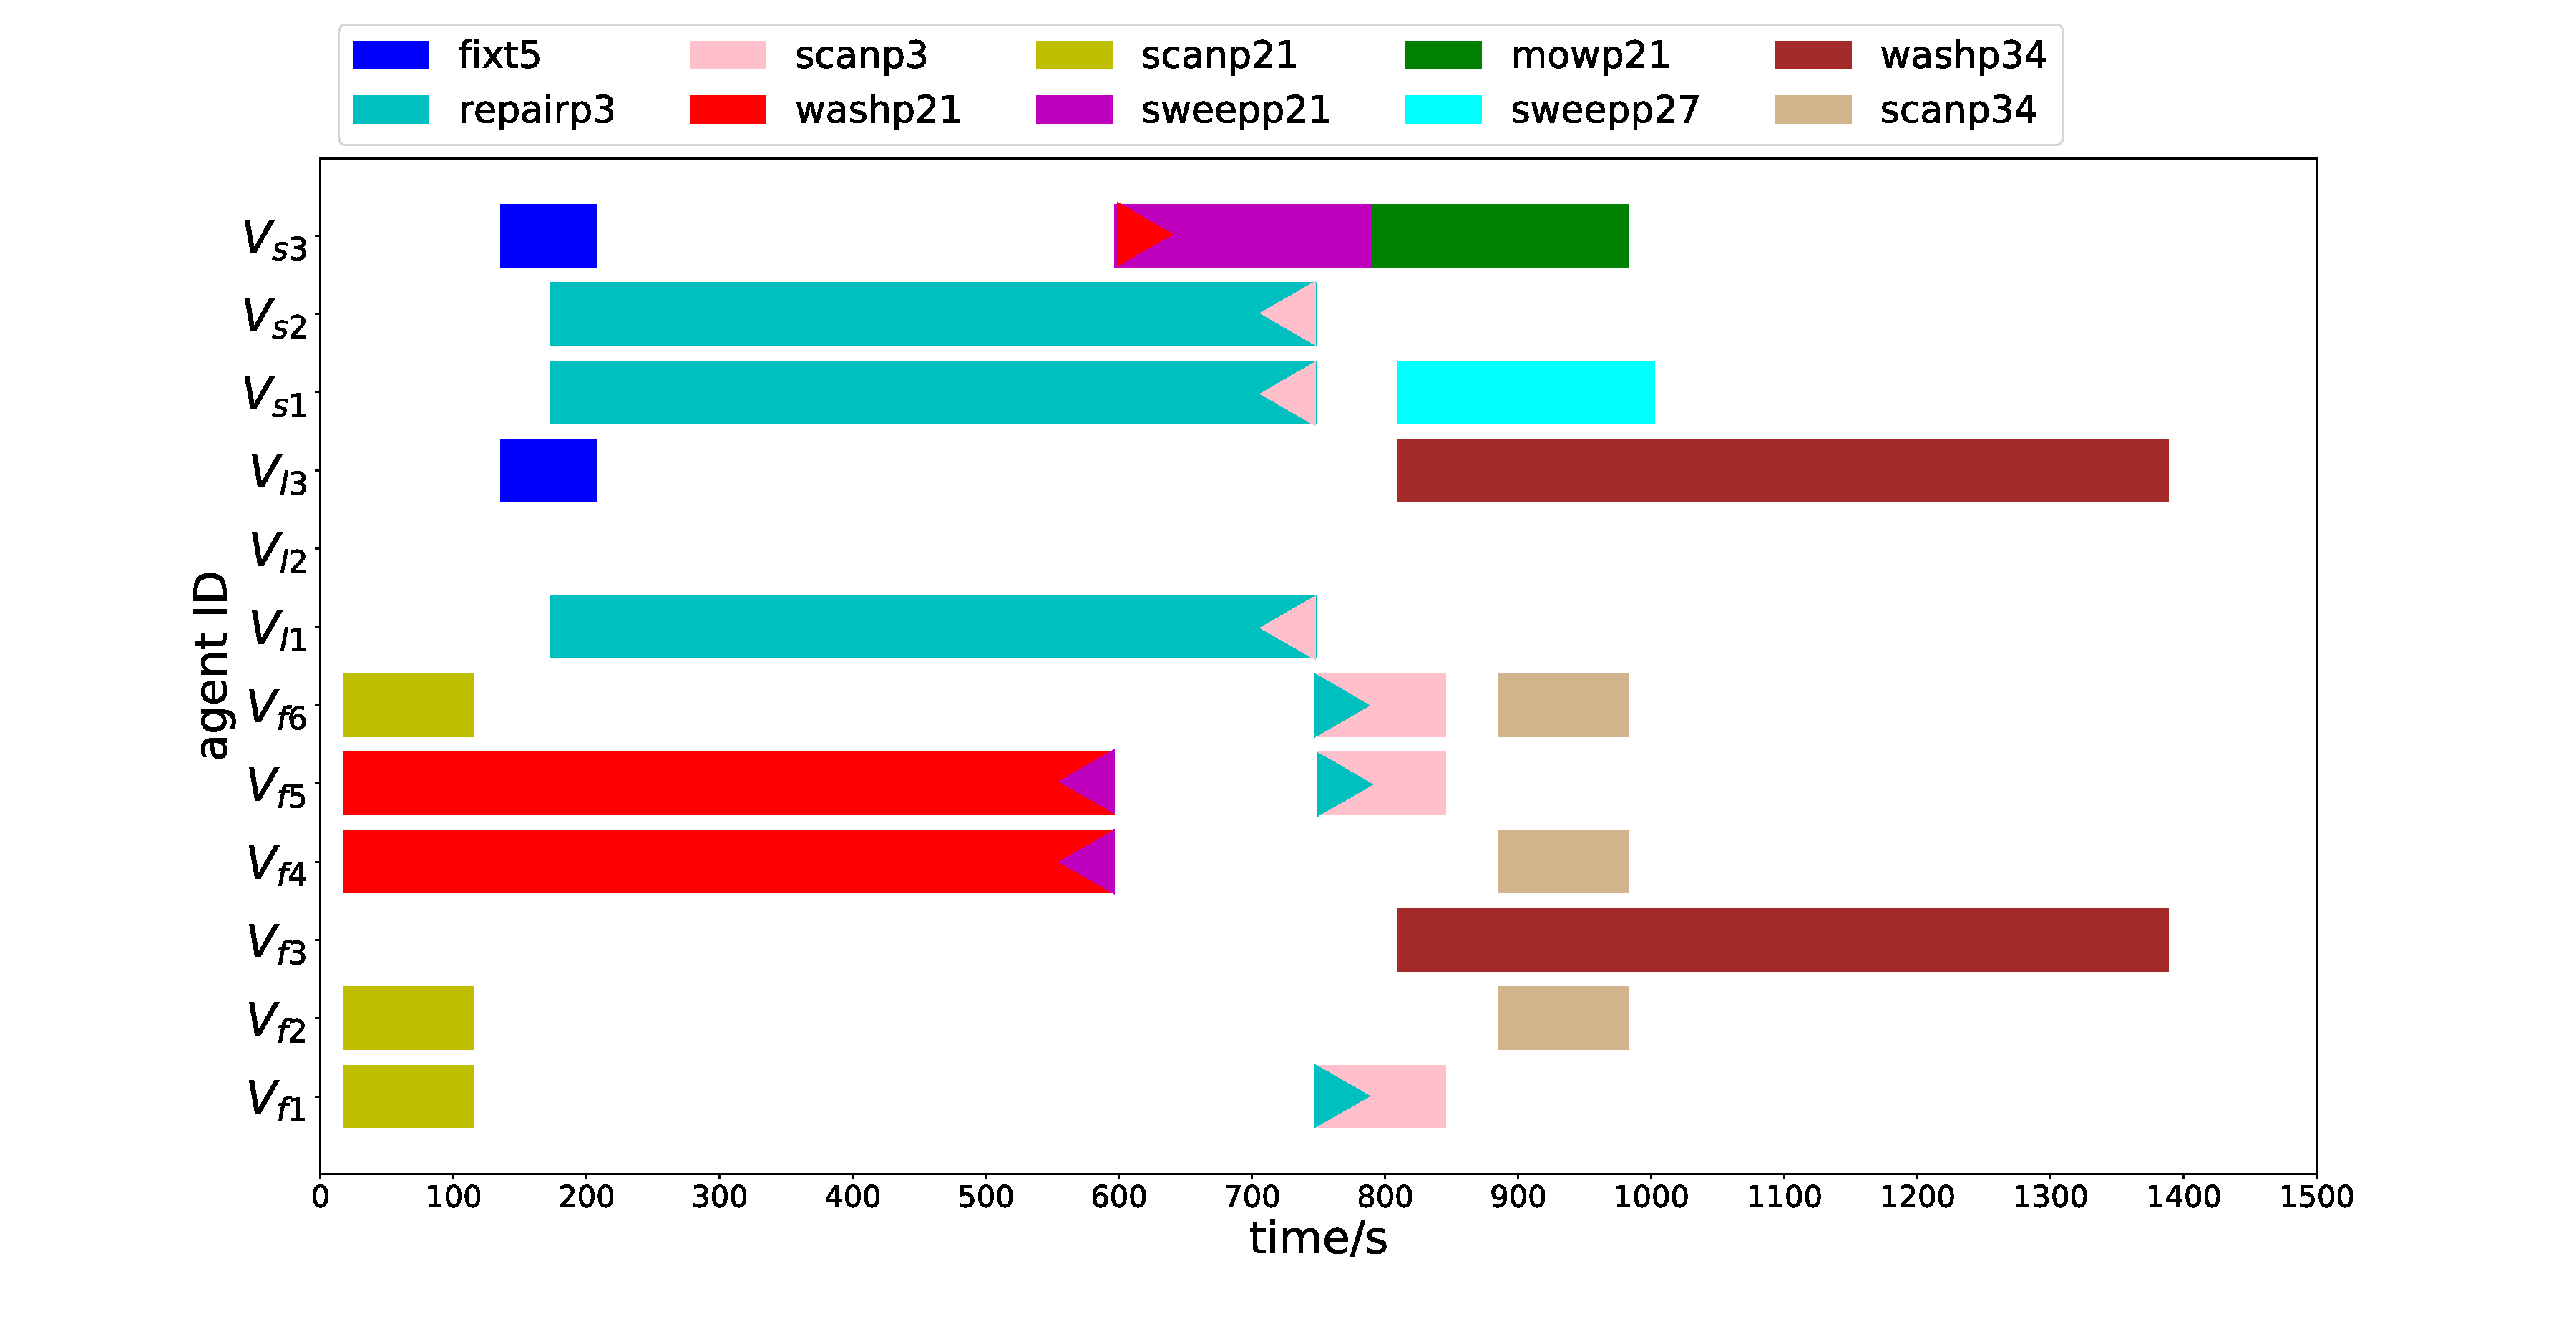
\includegraphics[height =0.5\textwidth]{figures/simulation/taskfinal/gantt_sim.pdf}

%% \end{minipage}%
%%    \centering %
%%    \label{Gantt_graph}
%% \caption{ Gantt graph of offline planning. }
%% \end{figure}
%% %==============================

%==============================
\subsubsection{Online Adaptation}\label{subsubsec:exp-adapt}
In this subsection, we simulate
two practical scenarios to validate the proposed online adaptation algorithm:
(i) fluctuations in the execution time of subtasks;
(ii) agent failures during online execution,

First of all, we artificially change the executing time of certain subtasks.
For instance, the executing time of the maintenance tasks for smaller panels
is reduced in comparison to the large panels, e.g., the execution time
of $\texttt{wash}_{\texttt{p}_{34}}$ are reduced to $141s$ from $565s$, as the size
of $\texttt{p}_{34}$ is $25\%$ of~$\texttt{p}_{10}$. The transfer time
between different regions will be disturbed. The proposed online synchronization method in
 Sec.~\ref{subsubsec:uncertain} is applied during execution to dynamically accommodate these fluctuations.
 As shown in Fig.~\ref{fig:task2-bnb}, $V_{s_1}, V_{s_2}$ arrive $p_3$ first
and then begin ``communicate with collaborate leader" until leader $V_{l_1}$ arrives $p_3$ and returns the message ``synchronization begins". After finish task $\texttt{scan}_{\texttt{p}_{21}}$,
  agent $V_{f_2} $ go to the proper place quickly but cannot start $\texttt{scan}_{\texttt{p}_{34}}$ as its cooperators are not arrived
  and the related partial orders are also not satisfied.
  Thus, it turns to the states of ``communicate with other leader for \texttt{start} and \texttt{stop} messages" and "communicate with collaborate leader" .


%==============================
\begin{table}[t]\footnotesize
  \centering
  \begin{threeparttable}
	\caption{Scalability analyses of the proposed method\tnote{1}}
	\label{table:more-agents}
  \begin{tabular}{|c|c|c|c|}\hline
     \begin{tabular}{@{}c@{}} System \\ $(V_f,V_s,V_l)$\end{tabular}
    &  $t_{\varphi_1}\,[s]$
    &  $t_{\varphi_2}\,[s]$
    &  $t_{\varphi_3}\,[s]$  \\[0.5ex] \hline
		$(8,4,4)$ & $0.13,5.9$ &$0.14,1.08$ & $0.23,4.81$  \\[0.5ex]
		$(12,6,6)$ & $0.15,4.6$  & $0.08,1.85$ & $0.22,5.23$ \\[0.5ex]
		$(16,8,8)$  & $0.13,5.0$  & $0.10,1.56$ & $0.21,4.33$ \\[0.5ex]
		$(20,10,10)$  & $0.53,8.4$ & $0.09,2.11$ & $0.58,6.20$  \\[0.5ex] \hline
		R-Poset analysis  & $64.4,71.1$ &$8.4,37.9$ & $136.4,552.5$ \\ [0.5ex]
    \hline
  \end{tabular}
  \begin{tablenotes}
  \item[1] System size is given by the number of different types of agents.
          The associated solution time is measured by two time stamps: 1) when the first solution or poset is returned; 
          2) when the optimal solution or the best poset with largest language is returned.
  \end{tablenotes}
\end{threeparttable}
\end{table}
%==============================

Secondly, more severe scenarios are simulated where agents break down
during task execution and thus are removed from the team.
More specifically, vehicle~$V_{f_4}$ breaks down at~$250s$, $V_{l_1},\, V_{s_3}$ break
down at~$600s$ during the execution of $\varphi_1$.
Consequently, as shown in Fig.~\ref{fig:task2-bnb}, $\texttt{wash}_{\texttt{p}_{21}}$
is re-assigned to other agent as one of its cooperaters $V_{f_4}$ is failed. Subtask
$\texttt{repai}$$\texttt{r}_{\texttt{p}_{3}}$ is continuing as its cooperation situation and partial relations
are still satisfied. As described in Sec.~\ref{subsubsec:failure},
the set of unfinished tasks is re-assigned to the remaining agents by re-identifying
the current node in the BnB search tree and continue the planning process.
It can be seen that no subtasks are assigned to~$V_{f_4}$ anymore in the updated assignment.
Then, as $V_{l_1},\, V_{s_3}$ break down at $600s$, the execution of subtask~$\texttt{repair}_{\texttt{p}_{3}}$
is interrupted. It is executed again by vehicles~$V_{l_2}$ and $V_{s_1},V_{s_3}$ at~$1222s$.
In the same way, the unfinished subtasks are re-assigned to the remaining agents.
It is worth noting that the partial ordering constraints are respected at all
time during the adaptation.
For instance, $V_{f_1}$ cannot execute the subtask~$\texttt{wash}_{\texttt{p}_{34}}$
before~$\texttt{mow}_{\texttt{p}_{21}}$ is started,
as~$\texttt{mow}_{\texttt{p}_{21}}\preceq_\varphi\texttt{wash}_{\texttt{p}_{34}}  $ holds.
All subtasks are fulfilled at~$2109s$, despite of the above contingencies. 
The trajectories of the agents are showed in Fig.~\ref{fig:workspace}.



%==============================
\subsubsection{Scalability Analysis}\label{subsubsec:scalable}
To further validate the scalability of the proposed methods,
the following tests are performed:
(i) the same task with increased team sizes,
e.g., $16$, $24$, $32$ and $40$;
(ii) more LTL formulas with different structures.

As summarized in Table~\ref{table:more-agents},
as the system size is increased from~$8$ to $40$,
the computation time to obtain the \emph{first}
solution for task $\varphi_1$ remains almost unchanged,
while the time taken to compute the optimal value increases slightly.
This result verifies that the proposed anytime algorithm is beneficial
especially for large-scale systems, as it can returns a high-quality solution fast,
and close-to-optimal solutions can be returned as time permits.
Secondly, more tasks $\varphi_2,\varphi_3$ are considered as follows:
\begin{equation}\footnotesize
\label{eq:task2}
\begin{aligned}
\varphi_2 = &\Diamond (\texttt{wash}_{\texttt{p}_{11}} \land \lnot\texttt{scan}_{\texttt{p}_i} \wedge\Diamond \texttt{scan}_{\texttt{p}_{11}}\wedge \Diamond ((\texttt{mow}_{\texttt{p}_{11}}\quad\quad\quad \\
&\wedge\lnot \texttt{wash}_{\texttt{p}_{11}} ) \wedge\Diamond (\texttt{sweep}_{\texttt{p}_{11}} \land \lnot\texttt{mow}_{\texttt{p}_{11}} )))\wedge\\
&\Diamond (\texttt{temp}_{\texttt{p}_{25}} \land \Diamond \texttt{repair}_{\texttt{p}_{25}}\wedge \Diamond ((\texttt{scan}_{\texttt{p}_{25}}\wedge\\
&\lnot \texttt{wash}_{\texttt{p}_{25}} ) \wedge\Diamond (\texttt{sweep}_{\texttt{p}_{25}} \land \lnot{\texttt{p}_{26}} ))) \wedge  \Diamond
\texttt{temp}_{\texttt{t}_4},
\end{aligned}
\end{equation}

\begin{equation}\footnotesize
\label{eq:task3}
\begin{aligned}
\varphi_3 = &\Diamond (\texttt{temp}_{\texttt{p}_{25}} \land\Diamond \texttt{repair}_{\texttt{p}_{25}}
\wedge \Diamond ((\texttt{scan}_{\texttt{p}_{25}}\wedge
\lnot \texttt{wash}_{\texttt{p}_{25}} ) \\
&\wedge\Diamond (\texttt{sweep}_{\texttt{p}_{25}} \land \lnot{\texttt{p}_{26}} ))) \wedge  \Diamond
\texttt{temp}_{\texttt{t}_4}
\wedge  \Diamond (\texttt{sweep}_{\texttt{p}_{8}}\\& \wedge \Diamond \texttt{wash}_{\texttt{p}_{8}} )\land \Diamond \texttt{repair}_{\texttt{p}_4} \bigcirc \lnot \texttt{p}_5 \wedge \Diamond ( \texttt{sweep}_{\texttt{p}_{8}}\\
& \wedge \lnot \texttt{wash}_{\texttt{p}_{8}} \wedge\Diamond
\texttt{scan}_{\texttt{p}_{8}} )\wedge \lnot \texttt{temp}_{\texttt{t}_4} \,U \, \texttt{fix}_{\texttt{t}_{4}},
\end{aligned}
\end{equation}
where~$\mathcal{B}_{\varphi_2}$ contains $216$ states
	 and~$\mathcal{B}_{\varphi_3}$ contains~$970$ states.
	As summarized in Table~\ref{table:more-agents} , the computation time of
	 both R-posets and tasks assignment are increased significantly, as the task becomes more
	 complex.
	 However, the time when the first solution is obtained in tasks assignment does not monotonically increase due to
	 the polynomial complexity of upper bound method.





%==============================
\subsubsection{Comparison}\label{subsubsec:compare}
The proposed method is compared against several
state-of-the-art methods in the literature.
More specifically, four methods below are compared:

\textbf{Prod}: the standard solution~\citep{baier2008principles}
that first computes
the Cartesian products of all agent models,
then computes the product B\"uchi automaton,
and searches for the accepting run within.
As the brute-force method,
it is well-known to suffer from complexity explosion.

\textbf{Milp}: the optimization-based solution that
formulates the assignment problem of R-posets as a MILP,
the compute optimal assignment similar
to~\citep{luo2021temporal, jones2019scratchs},
i.e., instead of the search method.
The partial relations are formulated as constraints
in the program.
An open source solver GLPK~\citep{makhorin2008glpk} is used.

\textbf{Samp}: the sampling based method proposed
in~\citep{kantaros2020stylus}.
Compared with the product-based methods, it does not pre-compute
the complete system model. Instead, it relies on a sampling strategy
to explore only relevant search space.
However, since it does not support collaborative actions natively,
we modify the definition of transitions there slightly.

\textbf{Decomp}: the task assignment strategy proposed
in~\citep{schillinger2018simultaneous}.
As discussed earlier in Sec.~\ref{sec:introduction},
the proposed task decomposition strategy only allows completely
independent subtasks.
Furthermore, since it does not support collaborative actions,
collaborative subtasks are decomposed manually.
%==============================
\begin{table}[t]\footnotesize
  \centering
  \begin{threeparttable}
	\caption{Comparisons to other methods\tnote{1}}
	\label{table:compare_time}
	\begin{tabular}{|c|c|c|c|c|c|}\hline
	   Method &  $t_{\texttt{fir}}\, [s]$
          &  $t_{\texttt{opt}}\, [s]$
	  &  $t_{\texttt{fin}}\,[s]$ & $T_{\texttt{obj}}\,[s]$
          &  $N_{\texttt{sync}}$ \\ \hline
		\multirow{2}{*}{\textbf{Prod}}& $\infty$ & $\infty$ & $\infty$ & -- & -- \\
                 & $\infty$ & $\infty$ & $\infty$ & -- & -- \\
                \hline
		\multirow{2}{*}{\textbf{Milp}} & 2069.27 & 2069.27 & 2069.27 & 1058.47 & -- \\
                &$\infty$ &$\infty$ & $\infty$ & -- & --  \\
                \hline
		\multirow{2}{*}{\textbf{Samp}} & 328.59 & 1838.96 & $\infty$ & 1968.03 & 24 \\
                 & 3280.68 &  16294.30 & $\infty$ & 1968.03 & 24 \\
                \hline
		\multirow{2}{*}{\textbf{Decomp}} & 580.16 & 580.16 & 4581.3 & 1266.99 & 0 \\
		 & 1151.24 & 1151.24 & 5082.07 & 1267.00 & 0 \\
                \hline
		\multirow{2}{*}{\textbf{Ours}} & 24.81 & 25.26 & $\infty$ & 1058.47 & 8 \\
                 & 28.12 & 37.40 & $\infty$ & 1058.47 & 8 \\
		\hline
	\end{tabular}
  \begin{tablenotes}
  \item[1] $t_\texttt{fir}$ is the time to get the first solution; $t_\texttt{opt}$ 
	the time to get the optimal solution; $t_\texttt{fin}$ the time to complete the search; $T_\texttt{obj}$ the makespan; and $N_\texttt{sync}$ the number of synchronization during execution.
  \end{tablenotes}
\end{threeparttable}
\end{table}
%==============================

Comparisons are performed under different system sizes,
namely, $12$ and $24$ agents, to compare not only efficiency but also scalability.
To begin with, the nominal system of~$12$ agents under task~$\varphi_2$ is considered.
The above four methods are used to solve the same planning problem. The results are 
summarized in Table~\ref{table:compare_time}.
Since the methods \textbf{Prod}, \textbf{Milp} and \textbf{Decomp} are not
anytime, the time to obtain  the first solution equals to the time
when the optimal solution is obtained.
It can be seen that \textbf{Prod} fails to generate any solution
within~$11h$ as the system-wide product automata for both cases
has more than $10^{19}$ states.
The \textbf{Milp} method is only applicable for small-scale systems,
which returns the optimal solution in~$0.5h$ but fails to
return any solution within~$16h$ for the large-scale case.
The \textbf{Samp} method has the anytime property but it takes ten times
more time to generate
the first  solution, compared with our method.
In addition, since the subtasks are executed in sequence,
the actual time of task completion is significantly longer.
The \textbf{Decomp} method can solve both problems but the overall time
for task completion is longer than our results,
which matches our analyses in Remark~\ref{remark:compare-poset}.
In comparison, our method returns the first solution for both cases in less
than~$30s$ and the optimal solution within another~$10s$.
It can be seen that the task completion time remains the same for both cases.

Lastly, the last column in Table~\ref{table:compare_time} compares the number
of synchronizations required during execution.
Although the same solution is obtained, the \textbf{Milp} method requires more
synchronization than our method.
This is because our method requires only synchronization for relations within the
R-posets, rather than all consecutive subtasks.
The \textbf{Prod} and \textbf{Samp} methods require more synchronization due to
their fully sequential execution,
while the \textbf{Decomp} method requires no synchronization as
the local subtasks of each agent are independent.
